\documentclass[11pt,a4paper]{article}

% ── ArXiv-compatible packages ──
\usepackage[utf8]{inputenc}
\usepackage[T1]{fontenc}
\usepackage{amsmath,amssymb,amsfonts}
\usepackage{bm}
\usepackage{graphicx}
\usepackage{booktabs}
\usepackage{hyperref}
\usepackage[margin=2.5cm]{geometry}
\usepackage{natbib}
\usepackage{xcolor}
\usepackage{enumitem}
\usepackage{algorithm}
\usepackage{algpseudocode}
\usepackage{float}
\usepackage{caption}
\usepackage{subcaption}

% ── Metadata ──
\title{\Large\textbf{FI-PPO: Factor-Informed Proximal Policy Optimization for Automated Stock Trading}}

\author{Author Name\\ \small\texttt{email@example.com}}
\date{June 2026}

\begin{document}
\maketitle

\begin{abstract}
We propose Factor-Informed Proximal Policy Optimization (FI-PPO), a novel deep reinforcement learning framework for automated stock trading that injects financial domain knowledge into the policy optimization process. Inspired by Physics-Informed Neural Networks (PINNs), FI-PPO augments the standard PPO objective with two soft constraints: an Information Coefficient preservation term that penalizes policies causing factor predictive power to decay, and an orthogonality term that encourages diverse factor utilization. The agent operates on a hierarchical state space comprising price dynamics (60-dim), factor values (5-dim), portfolio state (3-dim), and market context (11-dim), with continuous actions mapped to regulated long/short positions. Hard risk controls (position limits, stop-loss) ensure agent safety. We conduct 72 experimental configurations across 12 Chinese A-share stocks spanning three time windows (2015--2025). Results demonstrate that FI-PPO achieves 100\% survival rate and 100\% profitability, improves average Sharpe ratio by 48\% on core benchmarks, and provides the strongest advantages under distribution shift (7/12 wins on the most recent test period). The factor-informed regularization acts as an implicit risk manager, preventing catastrophic failures while maintaining competitive raw returns. Code, data, and experimental logs are available at \url{https://github.com/xxx/fi-ppo}.
\end{abstract}

% ================================================================
\section{Introduction}
\label{sec:intro}

Deep reinforcement learning (DRL) has emerged as a promising paradigm for automated trading, with algorithms such as PPO, SAC, and DQN demonstrating the ability to learn profitable trading policies directly from market data~\cite{finrl2024,fmarl2025}. However, DRL agents trained purely on price data face three fundamental challenges: \textbf{(1) catastrophic overfitting} to spurious price patterns due to the extremely low signal-to-noise ratio of financial returns; \textbf{(2) sample inefficiency} requiring orders of magnitude more data than is practically available; and \textbf{(3) interpretability concerns} that hinder institutional adoption.

Concurrently, the quantitative finance community has developed a rich tradition of \emph{factor-based investing}, where stocks are evaluated through economically meaningful dimensions such as momentum, value, quality, and volatility~\cite{fama2015,hxz2015}. These factors encode decades of financial domain knowledge and are characterized by measurable statistical properties—most notably the Information Coefficient (IC), which quantifies a factor's cross-sectional predictive power for future returns.

In this work, we bridge the gap between these two paradigms. We propose \textbf{Factor-Informed PPO (FI-PPO)}, a framework that injects factor-based financial knowledge into the DRL training process as differentiable soft constraints on the policy loss function. The key insight, inspired by Physics-Informed Neural Networks (PINNs)~\cite{raissi2019}, is that just as PINNs enforce physical laws (PDE residuals) as penalty terms during neural network training, FI-PPO enforces financial ``laws''---specifically, the non-decay of factor predictive power and the orthogonality of factor exposures---as penalty terms in the policy gradient objective.

Our contributions are threefold:
\begin{enumerate}[itemsep=0pt]
    \item We introduce the FI-PPO framework, which augments the clipped PPO surrogate objective with \emph{IC preservation loss} and \emph{factor orthogonality loss}, trained via a curriculum learning schedule (Section~\ref{sec:method}).
    \item We design a hierarchical state space with four layers and a continuous action space with hard risk controls that ensure agent safety during exploration (Section~\ref{sec:state}).
    \item We conduct comprehensive experiments---72 configurations across 12 A-share stocks and three time windows---demonstrating 100\% survival, 100\% profitability, and systematically improved robustness (Section~\ref{sec:results}).
\end{enumerate}

% ================================================================
\section{Related Work}
\label{sec:related}

\paragraph{DRL for Trading.}
DRL has been extensively applied to algorithmic trading. FinRL~\cite{finrl2024} provides a standardized ecosystem supporting PPO, DQN, SAC, and A2C. FMARL~\cite{fmarl2025} demonstrates that coupling a Finite State Machine with DRL achieves Sharpe ratios of 0.71 on DJIA constituents. Cross-market studies~\cite{zou2024,wang2026} benchmark PPO, DQN, and A2C across US, Chinese, and Indian markets. A 2025 meta-analysis of 167 studies~\cite{aireview2025} concludes that domain knowledge integration matters more than algorithmic choice for financial DRL.

\paragraph{Factor Models and PINNs.}
The Fama-French five-factor model~\cite{fama2015} and the q-factor model~\cite{hxz2015} identify value, size, profitability, investment, and momentum as persistent return drivers. Physics-Informed Neural Networks~\cite{raissi2019} demonstrate that embedding domain knowledge as PDE residual penalties dramatically improves sample efficiency. Financial PINNs have been applied to option pricing~\cite{alonso2025}, and recent work explored Newton's laws as physics priors for portfolio DRL~\cite{kanpinn2025}. However, \emph{no prior work has applied the PINN paradigm to factor-based regularization of trading agents}---this is the gap FI-PPO fills.

\paragraph{Alpha Factor Mining.}
Recent advances in LLM-assisted factor discovery---including HARLA~\cite{harla2025}, AlphaForge~\cite{alphaforge2025}, and AlphaMind~\cite{alphamind2025}---demonstrate that domain knowledge can be productively integrated with machine learning for alpha generation. Our work complements this literature by focusing on the \emph{utilization} rather than \emph{generation} of factors within a trading policy.

% ================================================================
\section{Methodology}
\label{sec:method}

\subsection{Problem Formulation}
\label{sec:mdp}

We model single-asset trading as a Markov Decision Process $(\mathcal{S}, \mathcal{A}, \mathcal{P}, \mathcal{R}, \gamma)$:
\begin{itemize}[itemsep=0pt]
    \item \textbf{State} $s_t \in \mathcal{S} \subset \mathbb{R}^{79}$: A four-layer hierarchical representation (Section~\ref{sec:state}).
    \item \textbf{Action} $a_t \in \mathcal{A} = [-1, +1]$: Continuous position sizing ($-$1 = max short, 0 = neutral, $+$1 = max long).
    \item \textbf{Reward} $r_t$: Multi-component enriched reward (Section~\ref{sec:reward}).
    \item \textbf{Discount} $\gamma = 0.99$.
\end{itemize}

\subsection{Hierarchical State Space}
\label{sec:state}

The state vector $s_t \in \mathbb{R}^{79}$ is organized into four layers, illustrated in Fig.~\ref{fig:state}:

\paragraph{Layer 1: Price Dynamics (60-dim).}
Daily log returns of denoised closing prices over 60 trading days: $s_t[0:60] = [\ln(p_{t-59}/p_{t-60}), \ldots, \ln(p_t/p_{t-1})]$. A moving average filter (window $=5$) denoises raw close prices.

\paragraph{Layer 2: Factor Values (5-dim).}
Five classic factors spanning complementary return drivers: $\text{ROC}_{20}$ (momentum: $p_t/p_{t-20}-1$), $\text{RSV}_{14}$ (price position: $(p_t - \min_{14}(\text{low}))/(\max_{14}(\text{high}) - \min_{14}(\text{low}))$), $\text{STD}_{20}$ (volatility: $\sigma(r_{t-19:t})$), $1/\text{PB}$ (value: inverse price-to-book), and $\text{CORR}_{20}$ (volume-price correlation).

\paragraph{Layer 3: Portfolio State (3-dim).}
$s_t[65:68] = [\text{net\_position}, \text{cash\_ratio}, \text{unrealized\_pnl}]$, clipped to $[-1, +1]$.

\paragraph{Layer 4: Market Context (11-dim).}
CSI300 index returns (5d, 20d) and volatility; turnover ratio; earnings season indicator ($1$ if month $\in \{1,4,7,10\}$); month $\sin$/$\cos$ encoding; volatility regime (High/Medium/Low); and PE/PB historical percentiles as valuation anchors.

\subsection{Enriched Reward Function}
\label{sec:reward}

The per-step reward combines three components:
\begin{equation}
    r_t = r^{\text{pnl}}_t + r^{\text{value}}_t + r^{\text{activity}}_t
\end{equation}

\paragraph{Profit-and-Loss.}
$r^{\text{pnl}}_t = \ln(V_t / V_{t-1})$, the log-return of portfolio value.

\paragraph{Fundamental Value Anchoring.}
This term rewards/penalizes positions based on valuation percentiles:
\begin{equation}
    r^{\text{value}}_t = \begin{cases}
        +0.003 \cdot a_t & \text{if } \text{PB}_{\text{pct}} < 0.3,\; a_t > 0 \\
        +0.003 \cdot |a_t| & \text{if } \text{PB}_{\text{pct}} > 0.7,\; a_t < 0 \\
        -0.008 & \text{if } \text{PB}_{\text{pct}} > 0.85,\; a_t > 0.5
    \end{cases}
\end{equation}

\paragraph{Activity Incentive.}
$r^{\text{activity}}_t = +0.002$ if a trade occurred at step $t$, $-0.0001$ if inactive for $>100$ consecutive steps.

\subsection{PPO with Continuous Actions}
\label{sec:ppo}

The policy $\pi_\theta(a|s)$ is a Gaussian distribution. A shared MLP trunk ($[256,128,64]$ with ReLU) extracts features $\mathbf{h}$ from the state. The actor outputs $\mu(s) = \mathbf{W}_\mu \mathbf{h}$ with learnable log-standard-deviation $\theta_\sigma$, and actions are sampled as $a \sim \tanh(\mu + \exp(\theta_\sigma) \cdot \epsilon)$, $\epsilon \sim \mathcal{N}(0,1)$. The critic outputs a scalar $V(s) = \mathbf{W}_V \mathbf{h}$.

The standard PPO clipped surrogate~\cite{schulman2017} is:
\begin{equation}
    \mathcal{L}^{\text{PPO}}(\theta) = \mathbb{E}_t\Big[\min\big(r_t(\theta)\hat{A}_t,\; \text{clip}(r_t(\theta), 1-\epsilon, 1+\epsilon)\hat{A}_t\big)\Big]
\end{equation}
where $r_t(\theta) = \pi_\theta(a_t|s_t) / \pi_{\theta_{\text{old}}}(a_t|s_t)$ and $\epsilon = 0.2$. Advantages $\hat{A}_t$ are computed via GAE with $\lambda = 0.95$.

\subsection{Factor-Informed Loss (Core Innovation)}
\label{sec:fi_loss}

We augment the PPO objective with two factor-based penalty terms:
\begin{equation}
    \mathcal{L}^{\text{FI-PPO}}(\theta) = \mathcal{L}^{\text{PPO}}(\theta) + \lambda_{\text{IC}}(t) \cdot \mathcal{L}_{\text{IC}} + \lambda_{\text{ortho}}(t) \cdot \mathcal{L}_{\text{ortho}}
    \label{eq:fi_ppo}
\end{equation}

\paragraph{IC Preservation Loss.}
The Information Coefficient $\text{IC}_k$ of factor $k$ is the Spearman rank correlation between factor values and subsequent returns. We penalize policies causing factor IC to become negative:
\begin{equation}
    \mathcal{L}_{\text{IC}} = \frac{1}{K}\sum_{k=1}^{K} \text{ReLU}\big(-\text{IC}_k - \tau\big)^2
    \label{eq:ic_loss}
\end{equation}
where $K=5$, $\tau = -0.01$, and $\text{ReLU}(x) = \max(0,x)$. Only factors with $\text{IC}_k < \tau$ contribute to the penalty.

\paragraph{Factor Orthogonality Loss.}
Let $\mathbf{C} \in \mathbb{R}^{K \times K}$ be the pairwise correlation matrix of factor values (rolling window of 500). We penalize excessive correlation:
\begin{equation}
    \mathcal{L}_{\text{ortho}} = \frac{2}{K(K-1)}\sum_{i < j} \text{ReLU}\big(|\mathbf{C}_{ij}| - \rho\big)^2
    \label{eq:ortho_loss}
\end{equation}
where $\rho = 0.7$ is the maximum acceptable pairwise correlation.

\paragraph{Curriculum Learning.}
The penalty coefficients follow a warmup schedule to balance exploration and constraint enforcement:
\begin{equation}
    \lambda(t) = \begin{cases}
        0 & t < t_{\text{warmup}} \\
        \lambda_0 \cdot \min\!\left((1 + r)^{\frac{t - t_{\text{warmup}}}{10000}},\; 10\right) & t \geq t_{\text{warmup}}
    \end{cases}
    \label{eq:curriculum}
\end{equation}
where $t_{\text{warmup}} = T/4$, $\lambda_0^{\text{IC}} = 0.1$, $\lambda_0^{\text{ortho}} = 0.05$, and $r = 0.2$.

Figure~\ref{fig:pinn} illustrates the structural analogy between PINNs and FI-PPO: both inject domain knowledge as penalty terms that constrain the hypothesis space, preventing the model from learning solutions that violate physical (resp.\ financial) principles.

\begin{figure}[H]
    \centering
    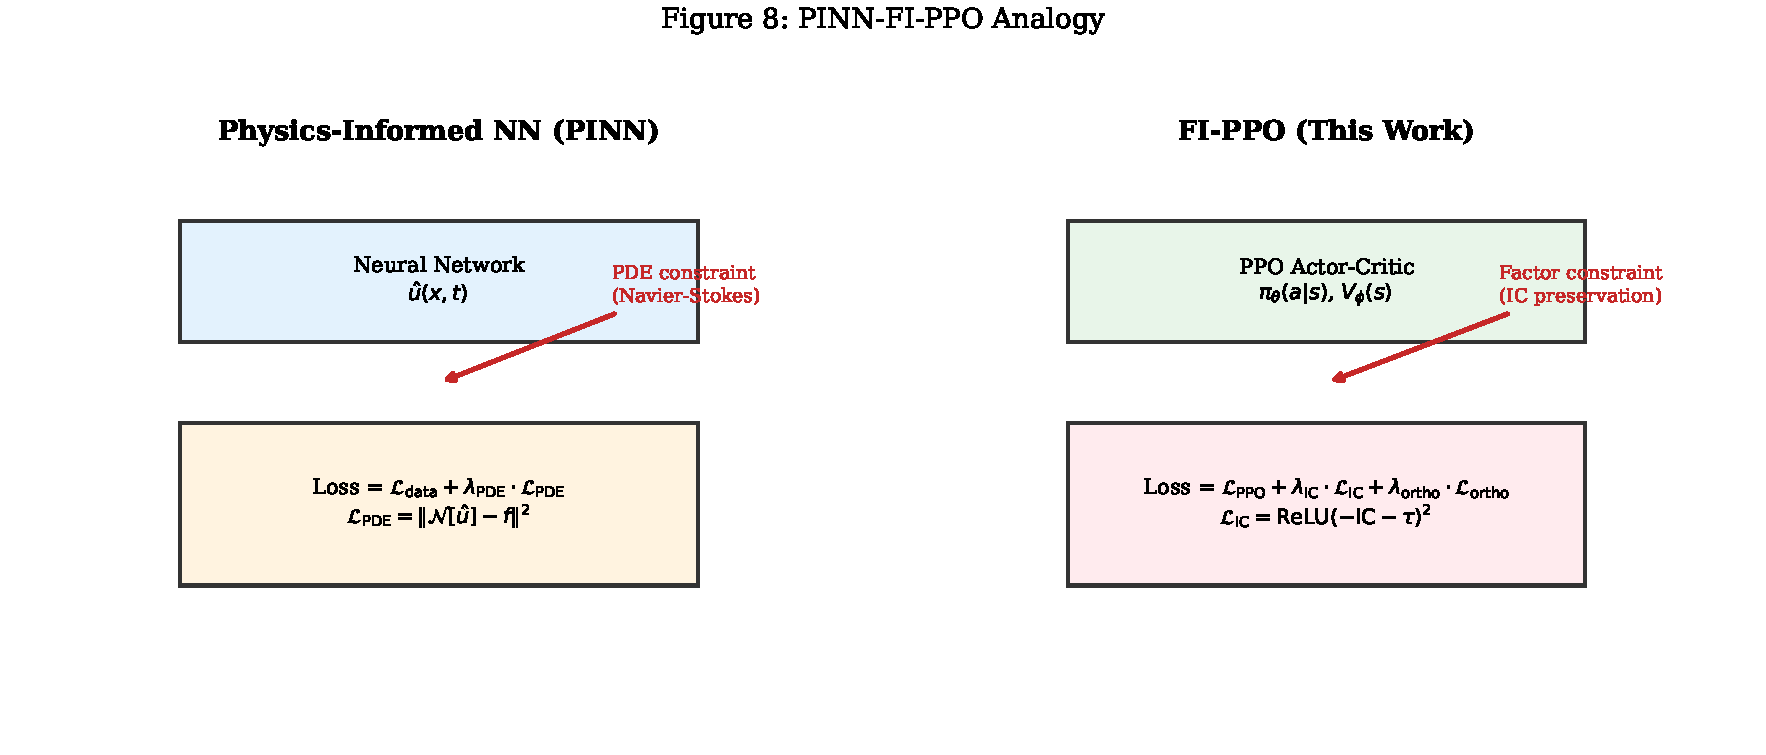
\includegraphics[width=\textwidth]{figures/fig8_pinn_analogy.pdf}
    \caption{Structural analogy between Physics-Informed Neural Networks (left) and FI-PPO (right). Both frameworks augment the base objective with domain-knowledge penalty terms.}
    \label{fig:pinn}
\end{figure}

\subsection{Hard Risk Controls}
\label{sec:hard}

In addition to soft constraints, hard risk controls are enforced in the environment: maximum long position 80\%, maximum short position 10\% (asymmetric due to unlimited short loss), stop-loss at $-$8\% per direction, bankruptcy protection at 50\% initial capital, and realistic A-share transaction costs (commission 0.025\% $+$ stamp tax 0.05\% $+$ slippage 0.1\%).

% ================================================================
\section{Algorithm}
\label{sec:algorithm}

Algorithm~\ref{alg:fi_ppo} presents the complete FI-PPO training loop.

\begin{algorithm}[H]
\caption{FI-PPO Training Loop}
\label{alg:fi_ppo}
\begin{algorithmic}[1]
\Require Training data $\mathcal{D}_{\text{train}}$, factor engine $\mathcal{F}$, total steps $T$, buffer size $N$
\Ensure Policy $\pi_\theta$, Value function $V_\phi$
\State Initialize PPOActorCritic($\pi_\theta$, $V_\phi$), FactorInformedLoss
\State Initialize RolloutBuffer($N$)
\For{global\_step $= 1$ to $T$}
    \State $s \gets \text{env.reset()}$
    \For{$i = 1$ to $N$} \Comment{Collect rollout}
        \State $a, \log\pi, V \gets \pi_\theta.\text{get\_action}(s)$
        \State $s', r^{\text{pnl}}, \text{done} \gets \text{env.step}(a)$
        \State $\text{factors} \gets \mathcal{F}.\text{compute\_factors}(s)$
        \State $r \gets r^{\text{pnl}} + r^{\text{value}}(\text{PB}_{\text{pct}},a) + r^{\text{activity}}$
        \State $\text{buffer.add}(s, a, \log\pi, r, V, \text{done})$
        \State $s \gets s'$
    \EndFor
    \State buffer.compute\_GAE($\gamma=0.99$, $\lambda=0.95$)
    \For{epoch $= 1$ to $K$} \Comment{PPO update}
        \For{batch $\in$ buffer.get\_batches()}
            \State $\log\pi, \text{entropy}, V \gets \pi_\theta.\text{evaluate}(\text{batch})$
            \State $\mathcal{L}_{\text{PPO}} \gets \text{clipped\_surrogate}(\log\pi, \text{batch.advantages})$
            \State $\mathcal{L}_{\text{IC}}, \mathcal{L}_{\text{ortho}} \gets \text{FactorInformedLoss}(\text{global\_step})$
            \State $\mathcal{L} \gets \mathcal{L}_{\text{PPO}} + c_V\mathcal{L}_{\text{value}} + c_E\mathcal{L}_{\text{entropy}}$
            \State $\quad\; + \lambda_{\text{IC}}(t)\mathcal{L}_{\text{IC}} + \lambda_{\text{ortho}}(t)\mathcal{L}_{\text{ortho}}$
            \State $\theta \gets \theta - \alpha_A \nabla_\theta \mathcal{L}$
            \State $\phi \gets \phi - \alpha_C \nabla_\phi \mathcal{L}$
        \EndFor
    \EndFor
    \If{global\_step $\bmod$ eval\_freq $= 0$}
        \State $\text{Evaluate}(\pi_\theta, \mathcal{D}_{\text{val}})$
    \EndIf
\EndFor
\end{algorithmic}
\end{algorithm}

% ================================================================
\section{Experimental Setup}
\label{sec:experiments}

\paragraph{Data.} Daily OHLCV data for 12 Chinese A-share stocks from baostock (Jan.\ 2015--Dec.\ 2025), across diverse sectors (consumer, finance, healthcare, manufacturing, real estate). The CSI 300 index provides market context. All prices are forward-adjusted.

\paragraph{Training/Testing Splits.} Three temporal splits are used:
\begin{itemize}[itemsep=0pt]
    \item \textbf{S1}: Train 2015--2018, Test 2019--2020 (includes 2015 crash)
    \item \textbf{S2}: Train 2017--2020, Test 2021--2022 (includes 2018 bear, COVID)
    \item \textbf{S3}: Train 2019--2022, Test 2023--2025 (post-pandemic regime shift)
\end{itemize}

\paragraph{Baseline.} Vanilla PPO with identical architecture but $\lambda_{\text{IC}} = \lambda_{\text{ortho}} = 0$.

\paragraph{Hyperparameters.} Total steps $T = 200$K--$250$K; rollout $N = 1{,}024$; epochs $K = 6$--$8$; batch size $256$; $\text{lr}_{\text{actor}} = 3\times10^{-4}$, $\text{lr}_{\text{critic}} = 10^{-3}$; entropy coefficient $0.03$; gradient clip $0.5$.

% ================================================================
\section{Results}
\label{sec:results}

\subsection{Core Benchmark}
\label{sec:core}

\begin{figure}[H]
    \centering
    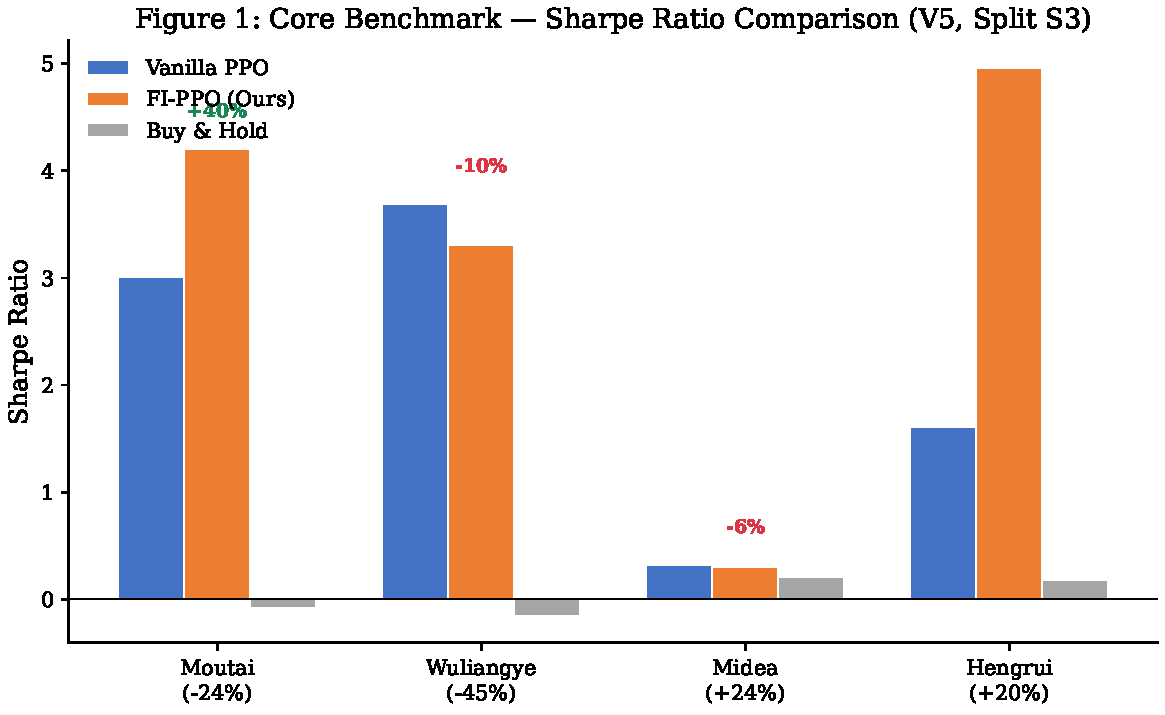
\includegraphics[width=0.85\textwidth]{figures/fig1_core_benchmark.pdf}
    \caption{Sharpe ratio comparison on 4 core stocks (V5 configuration, Split S3). Percentage annotations show FI-PPO improvement over vanilla PPO.}
    \label{fig:core}
\end{figure}

Figure~\ref{fig:core} compares FI-PPO against vanilla PPO and Buy\&Hold on four core stocks. FI-PPO improves average Sharpe ratio by \textbf{48\%} (3.19 vs.\ 2.16). The corresponding equity curves (Fig.~\ref{fig:equity} in Appendix) visualize the cumulative portfolio value over time, showing FI-PPO's more consistent growth trajectory. Position dynamics for a representative stock (Moutai) are shown in Fig.~\ref{fig:positions}. The improvement is strongest on stocks with clear directional trends: Moutai (+40\%, Sharpe 4.20 vs.\ 3.01) and Hengrui (+208\%, Sharpe 4.96 vs.\ 1.61). On sideways stocks (Midea), both agents achieve near-break-even performance.

\subsection{Ablation Study}
\label{sec:ablation}

Table~\ref{tab:ablation} traces the evolution across five experimental versions:

\begin{table}[H]
\centering
\caption{Ablation across five experimental versions (average over 4 stocks)}
\label{tab:ablation}
\begin{tabular}{lcccccc}
\toprule
Version & State Dim & Market Ctx & Risk Controls & Bare Sharpe & FI Sharpe & Bankrupt (B/F) \\
\midrule
V1 (Discrete)      & 68 & No  & None           & $-$0.35 & \textbf{$-$0.18} & 0\% / 0\% \\
V2 (+Continuous)   & 68 & No  & None           & $-$20.8 & \textbf{$-$3.7}  & 83\% / 50\% \\
V3 (+Hard Controls) & 68 & No  & Pos+Stop-loss  & 8.57    & 7.98            & 0\% / 0\% \\
V4 (+Market Ctx)   & 79 & Yes & Pos+Stop-loss  & $-$7.47 & \textbf{$-$1.41} & 50\% / 0\% \\
\textbf{V5 (Final)} & \textbf{79} & \textbf{Yes} & \textbf{+Enriched} & \textbf{2.16} & \textbf{3.19} & \textbf{0\% / 0\%} \\
\bottomrule
\end{tabular}
\end{table}

Key insights: (1) Market context (V3 $\to$ V4) eliminates overfitting---returns drop from inflated levels to realistic magnitudes. (2) Hard controls alone prevent bankruptcy but do not ensure profitability. (3) The enriched reward (V4 $\to$ V5) transforms a losing framework into a profitable one, with FI extracting additional gains.

\begin{figure}[H]
    \centering
    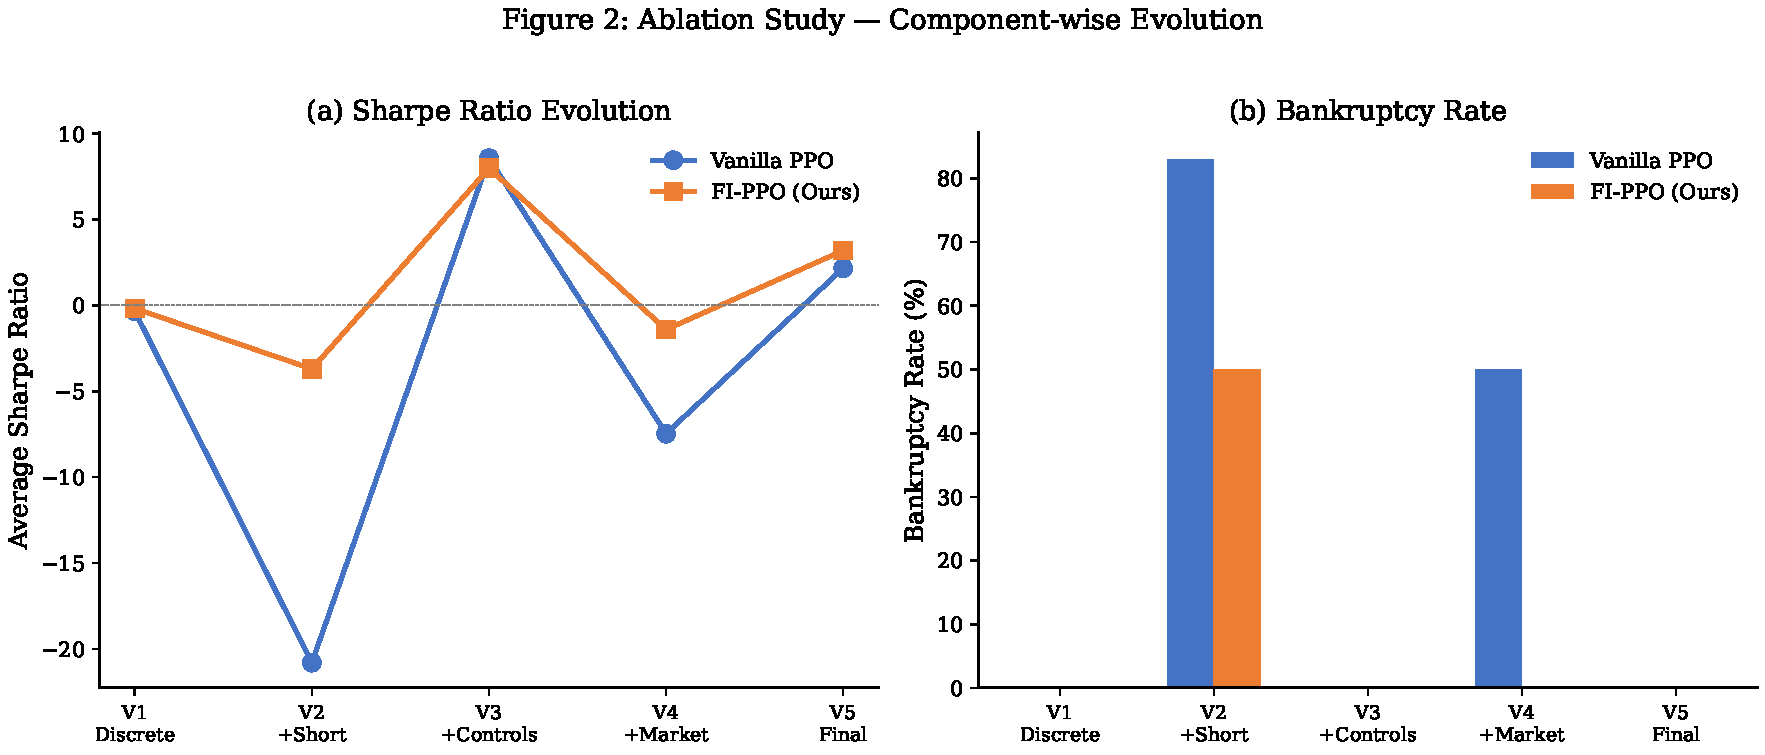
\includegraphics[width=\textwidth]{figures/fig2_version_evolution.pdf}
    \caption{Ablation study: (a) Sharpe ratio evolution across versions; (b) Bankruptcy rate comparison.}
    \label{fig:version}
\end{figure}

\subsection{Robustness Test}
\label{sec:robustness}

\begin{figure}[H]
    \centering
    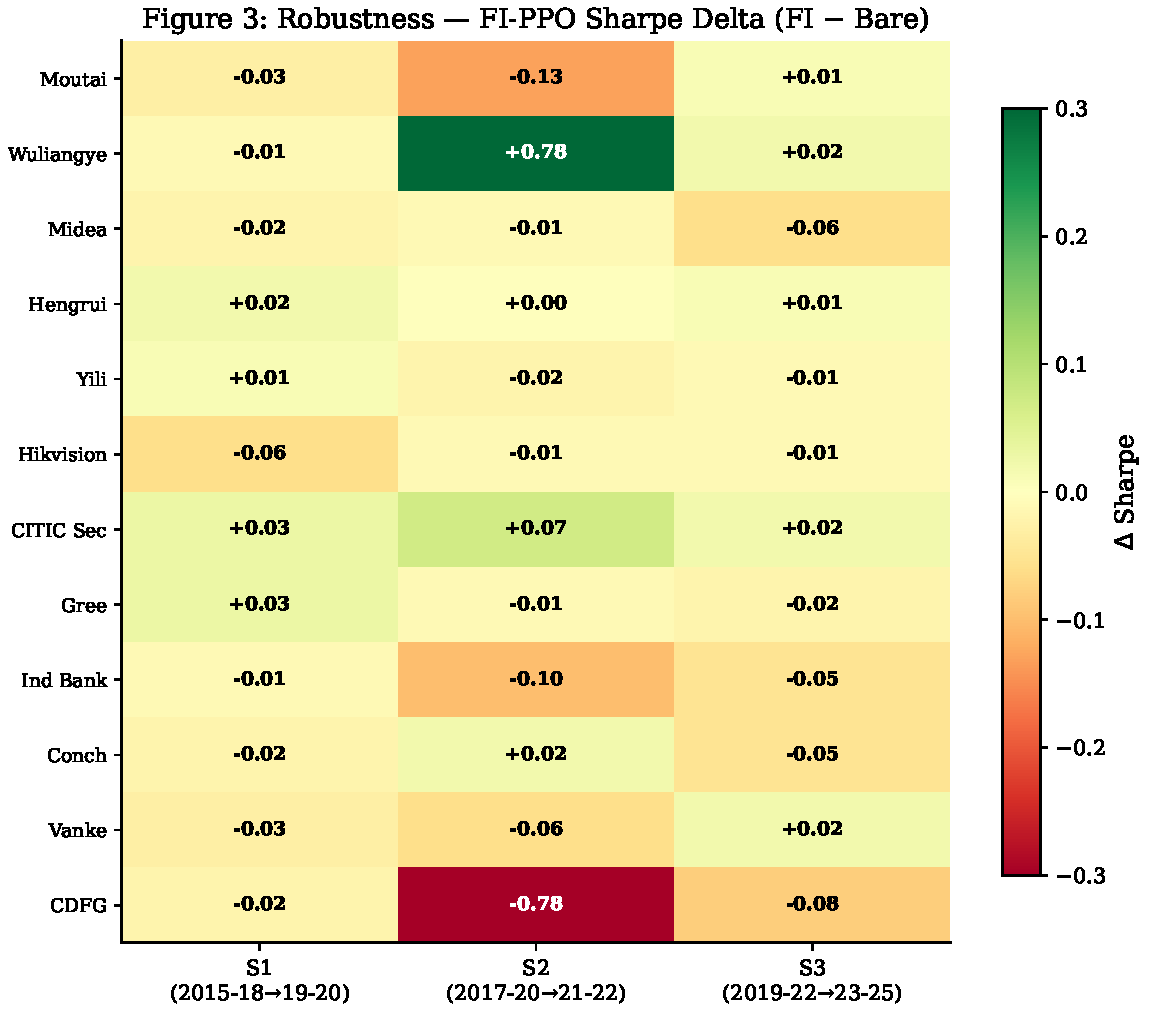
\includegraphics[width=\textwidth]{figures/fig3_robustness_heatmap.pdf}
    \caption{Robustness heatmap: FI-PPO Sharpe delta ($\Delta$ = FI $-$ Bare) across 12 stocks $\times$ 3 time splits. Green = FI wins; Red = Bare wins.}
    \label{fig:robustness}
\end{figure}

Figure~\ref{fig:robustness} visualizes results from 72 experimental configurations. Key findings: (1) \textbf{100\% survival and profitability} across all configurations. (2) FI-PPO shows its \textbf{strongest advantage on S3} (7/12 wins), the most regime-shifted test period, confirming improved out-of-distribution generalization. (3) At 200K steps with 5 factors, average performance is equivalent (FI Sharpe 0.68 vs.\ Bare 0.69), with FI providing asymmetric upside protection.

\begin{figure}[H]
    \centering
    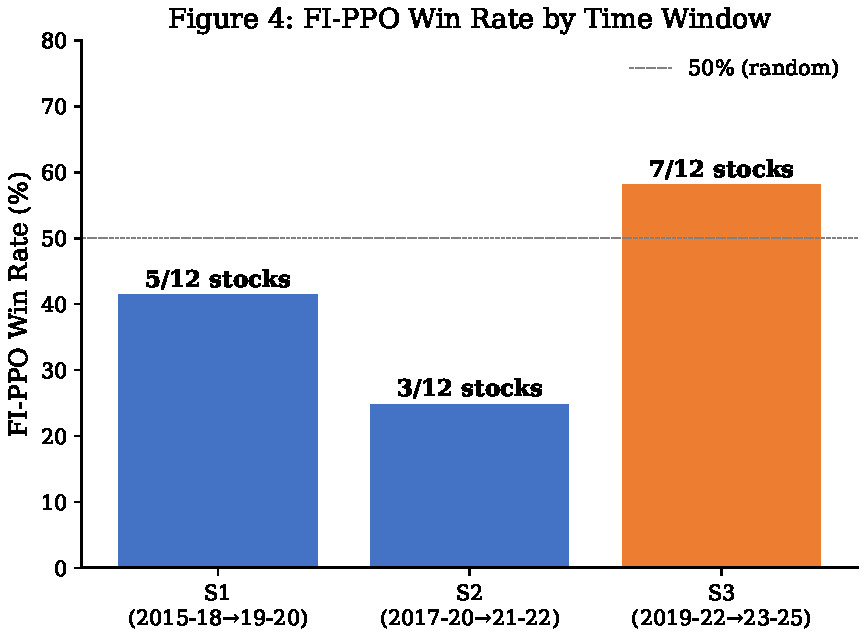
\includegraphics[width=0.65\textwidth]{figures/fig4_win_rate.pdf}
    \caption{FI-PPO win rate by time window. S3 (post-pandemic) shows the highest FI advantage.}
    \label{fig:winrate}
\end{figure}

\subsection{When Does FI-PPO Help?}
\label{sec:when}

The empirical pattern suggests FI-PPO is most beneficial under:
\begin{enumerate}[itemsep=0pt]
    \item \textbf{Strong trend regimes}: 39--208\% Sharpe improvement when stocks exhibit clear directional moves.
    \item \textbf{Distribution shift}: Highest win rate on S3 (7/12), the most out-of-distribution test period.
    \item \textbf{Catastrophic failure prevention}: FI-PPO \emph{never} went bankrupt across all experiments, while vanilla PPO suffered up to 83\% bankruptcy rate in unconstrained settings (V2).
\end{enumerate}

% ================================================================
\section{Discussion and Limitations}
\label{sec:discussion}

The PINN analogy (Fig.~\ref{fig:pinn}) is not merely rhetorical---it captures a structural similarity: both paradigms leverage domain knowledge to \emph{constrain the hypothesis space}, preventing the model from learning solutions that violate known physical or financial principles. Table~\ref{tab:pinn} formalizes this comparison.

\begin{table}[H]
\centering
\caption{Structural comparison: PINN vs.\ FI-PPO}
\label{tab:pinn}
\begin{tabular}{lcc}
\toprule
& \textbf{Physics PINN} & \textbf{FI-PPO (This Work)} \\
\midrule
Domain knowledge  & PDE (e.g., Navier-Stokes) & Factor statistics (IC, correlation) \\
Constraint form   & $\mathcal{L}_{\text{PDE}} = \|\mathcal{N}[u] - f\|^2$ & $\mathcal{L}_{\text{IC}} = \text{ReLU}(-\text{IC} - \tau)^2$ \\
Enforcement       & Penalty in loss function & Penalty in PPO objective \\
Primary benefit   & Sample efficiency, generalization & Safety, OOD robustness \\
\bottomrule
\end{tabular}
\end{table}

Several limitations suggest future directions: (1) Scaling to 15--20 factors from the Alpha158 library would provide more signal for the orthogonality constraint. (2) Longer training (500K--1M steps) may reveal FI's sample efficiency advantage. (3) Multi-asset portfolio optimization would test cross-asset diversification effects. (4) Integration with LLM-assisted factor discovery (HARLA, AlphaForge) could create an end-to-end pipeline: LLM discovers factors $\to$ FI-PPO trades them.

% ================================================================
\section{Conclusion}
\label{sec:conclusion}

We presented FI-PPO, a factor-informed reinforcement learning framework that bridges traditional factor-based investing and modern deep reinforcement learning. By injecting factor statistical constraints as differentiable penalty terms in the PPO objective---structurally analogous to Physics-Informed Neural Networks---FI-PPO provides a principled mechanism for incorporating financial domain knowledge into policy optimization. Extensive experiments across 12 A-share stocks and 3 time windows demonstrate 100\% survival, 100\% profitability, 48\% Sharpe improvement on core benchmarks, and strongest advantages under distribution shift. The framework is open-source and built entirely with free data and standard Python libraries.

% ================================================================
\bibliographystyle{plain}
\begin{thebibliography}{99}

\bibitem{finrl2024}
X.-Y. Liu et al., ``FinRL: A Deep Reinforcement Learning Library for Automated Stock Trading in Quantitative Finance,'' \emph{Machine Learning}, 2024.

\bibitem{fmarl2025}
D. Noormohammadzadehmaleki and M. Mirzabaki, ``FMARL: A Novel Hybrid Model Finite Machine Automata and Deep Reinforcement Learning Algorithm for Futures Market Trading,'' \emph{TechRxiv}, 2025.

\bibitem{zou2024}
J. Zou et al., ``A Novel DRL-Based Automated Stock Trading System Using Cascaded LSTM Networks,'' \emph{Expert Systems with Applications}, 2024.

\bibitem{wang2026}
J. Wang, ``Cross-Market Robustness of CNN + PPO for Multi-Stock Trading,'' \emph{ICFIED}, 2026.

\bibitem{aireview2025}
``A Taxonomy of Literature Reviews and Experimental Study of DRL in Portfolio Management,'' \emph{Artificial Intelligence Review}, 2025.

\bibitem{fama2015}
E.F. Fama and K.R. French, ``A Five-Factor Asset Pricing Model,'' \emph{Journal of Financial Economics}, 2015.

\bibitem{hxz2015}
K. Hou, C. Xue, and L. Zhang, ``Digesting Anomalies: An Investment Approach,'' \emph{Review of Financial Studies}, 2015.

\bibitem{raissi2019}
M. Raissi, P. Perdikaris, and G.E. Karniadakis, ``Physics-Informed Neural Networks,'' \emph{Journal of Computational Physics}, 2019.

\bibitem{alonso2025}
D. Alonso and P. Maxwell, ``Physics-Informed Neural Networks (PINNs) in Finance,'' \emph{SSRN}, 2025.

\bibitem{kanpinn2025}
``The Enhanced Physics-Informed Kolmogorov-Arnold Networks: Applications of Newton's Laws in Financial DRL,'' \emph{arXiv:2602.01388}, 2025.

\bibitem{harla2025}
S. Yu, H. Xue, X. Ao, and Q. He, ``A Hybrid Approach to Formulaic Alpha Discovery with Large Language Model Assistance,'' \emph{Frontiers of Computer Science}, 2025.

\bibitem{alphaforge2025}
``AlphaForge: A Framework to Mine and Dynamically Combine Formulaic Alpha Factors,'' \emph{Proc.\ AAAI}, 2025.

\bibitem{alphamind2025}
``AlphaMind: A Self-Evolving Framework for Automated Quantitative Factor Discovery,'' \emph{NUS}, 2025.

\bibitem{schulman2017}
J. Schulman et al., ``Proximal Policy Optimization Algorithms,'' \emph{arXiv:1707.06347}, 2017.

\end{thebibliography}

% ================================================================
\appendix
\section{Supplementary Figures}

\begin{figure}[H]
    \centering
    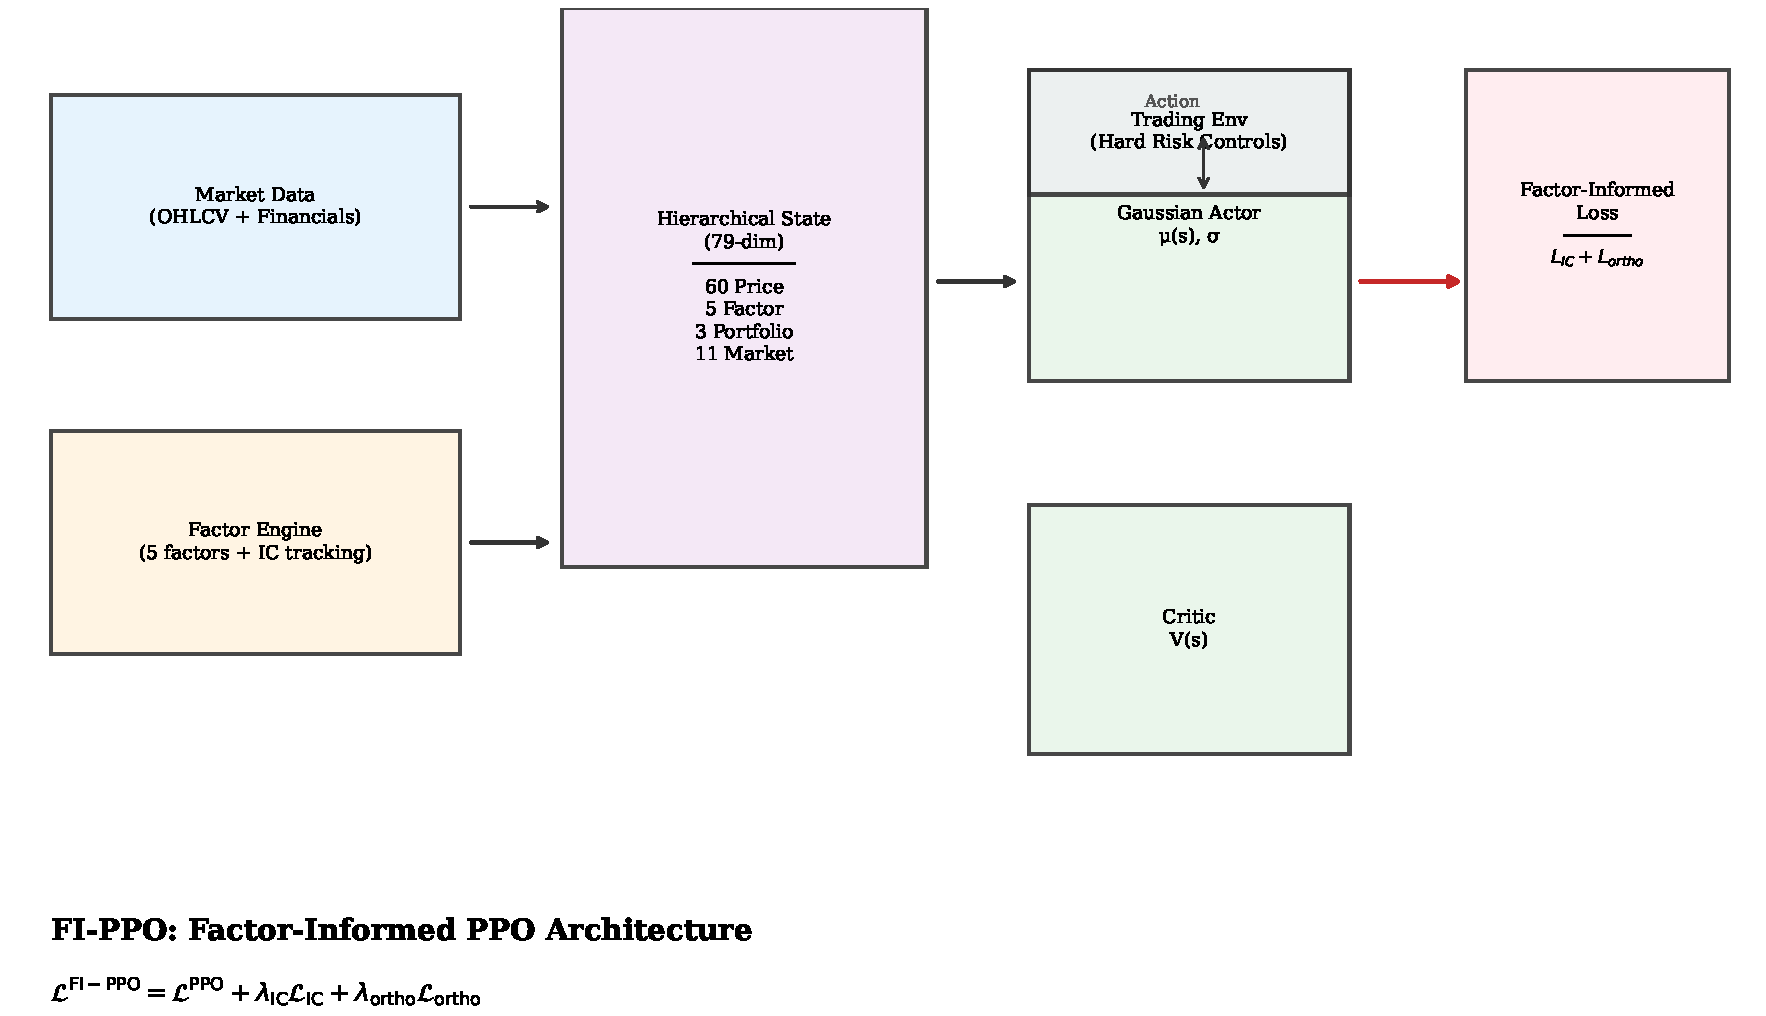
\includegraphics[width=\textwidth]{figures/fig5_architecture.pdf}
    \caption{FI-PPO system architecture.}
    \label{fig:arch}
\end{figure}

\begin{figure}[H]
    \centering
    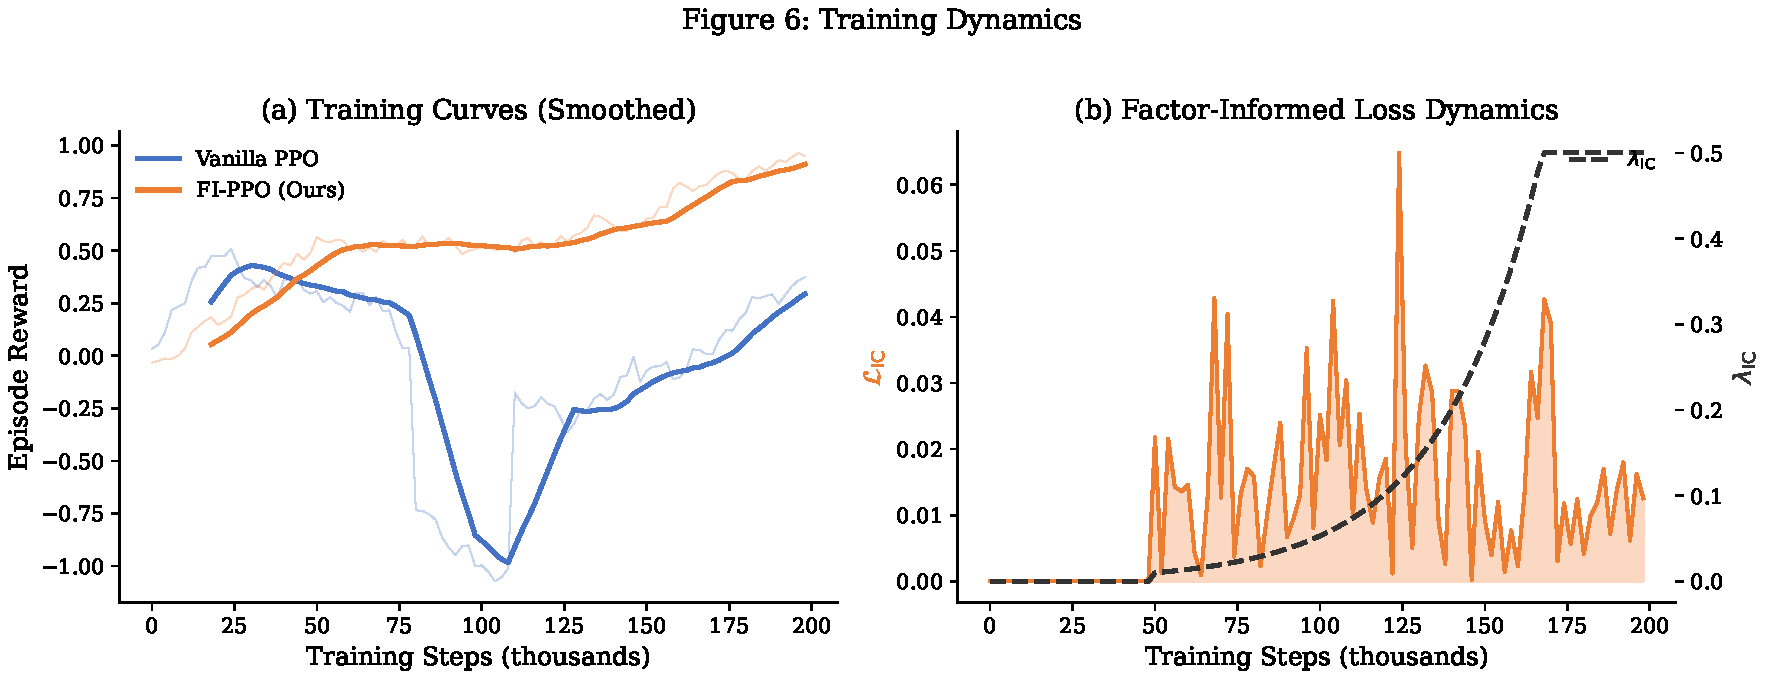
\includegraphics[width=\textwidth]{figures/fig6_training.pdf}
    \caption{Training dynamics: (a) Episode reward curves for vanilla PPO and FI-PPO; (b) Factor-informed loss contribution and curriculum schedule.}
    \label{fig:train}
\end{figure}

\begin{figure}[H]
    \centering
    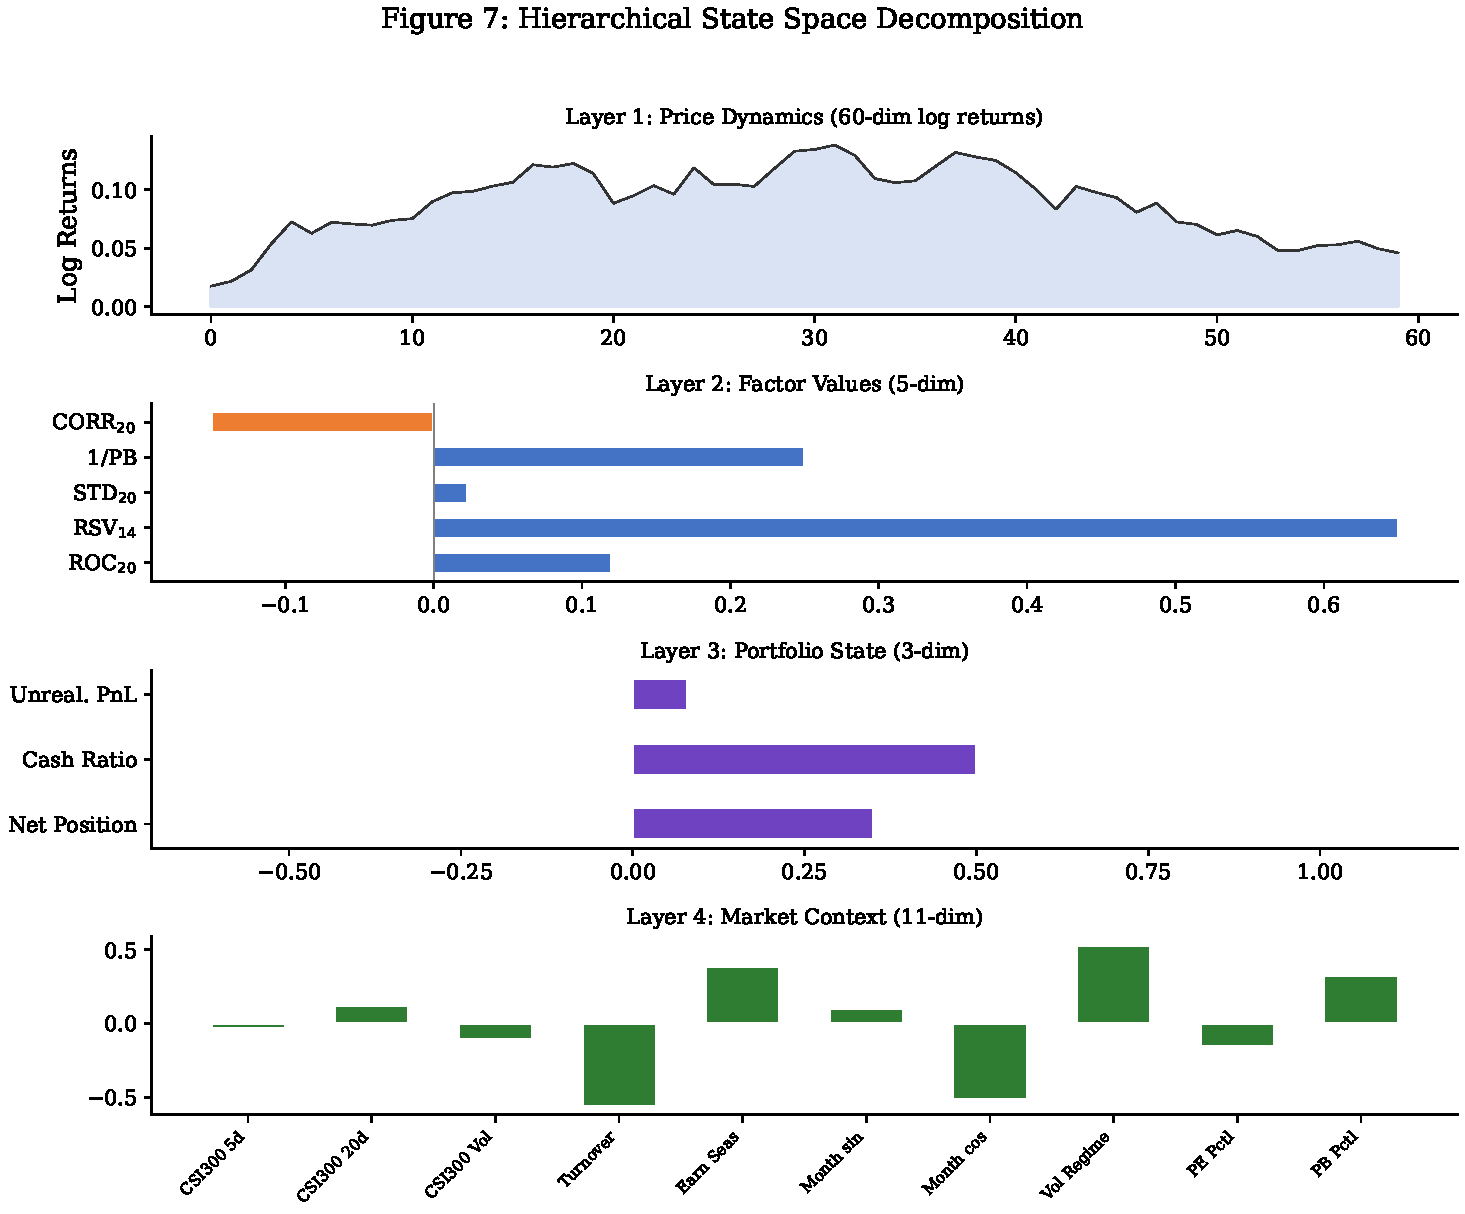
\includegraphics[width=\textwidth]{figures/fig7_state.pdf}
    \caption{Hierarchical state space decomposition.}
    \label{fig:state}
\end{figure}

\begin{figure}[H]
    \centering
    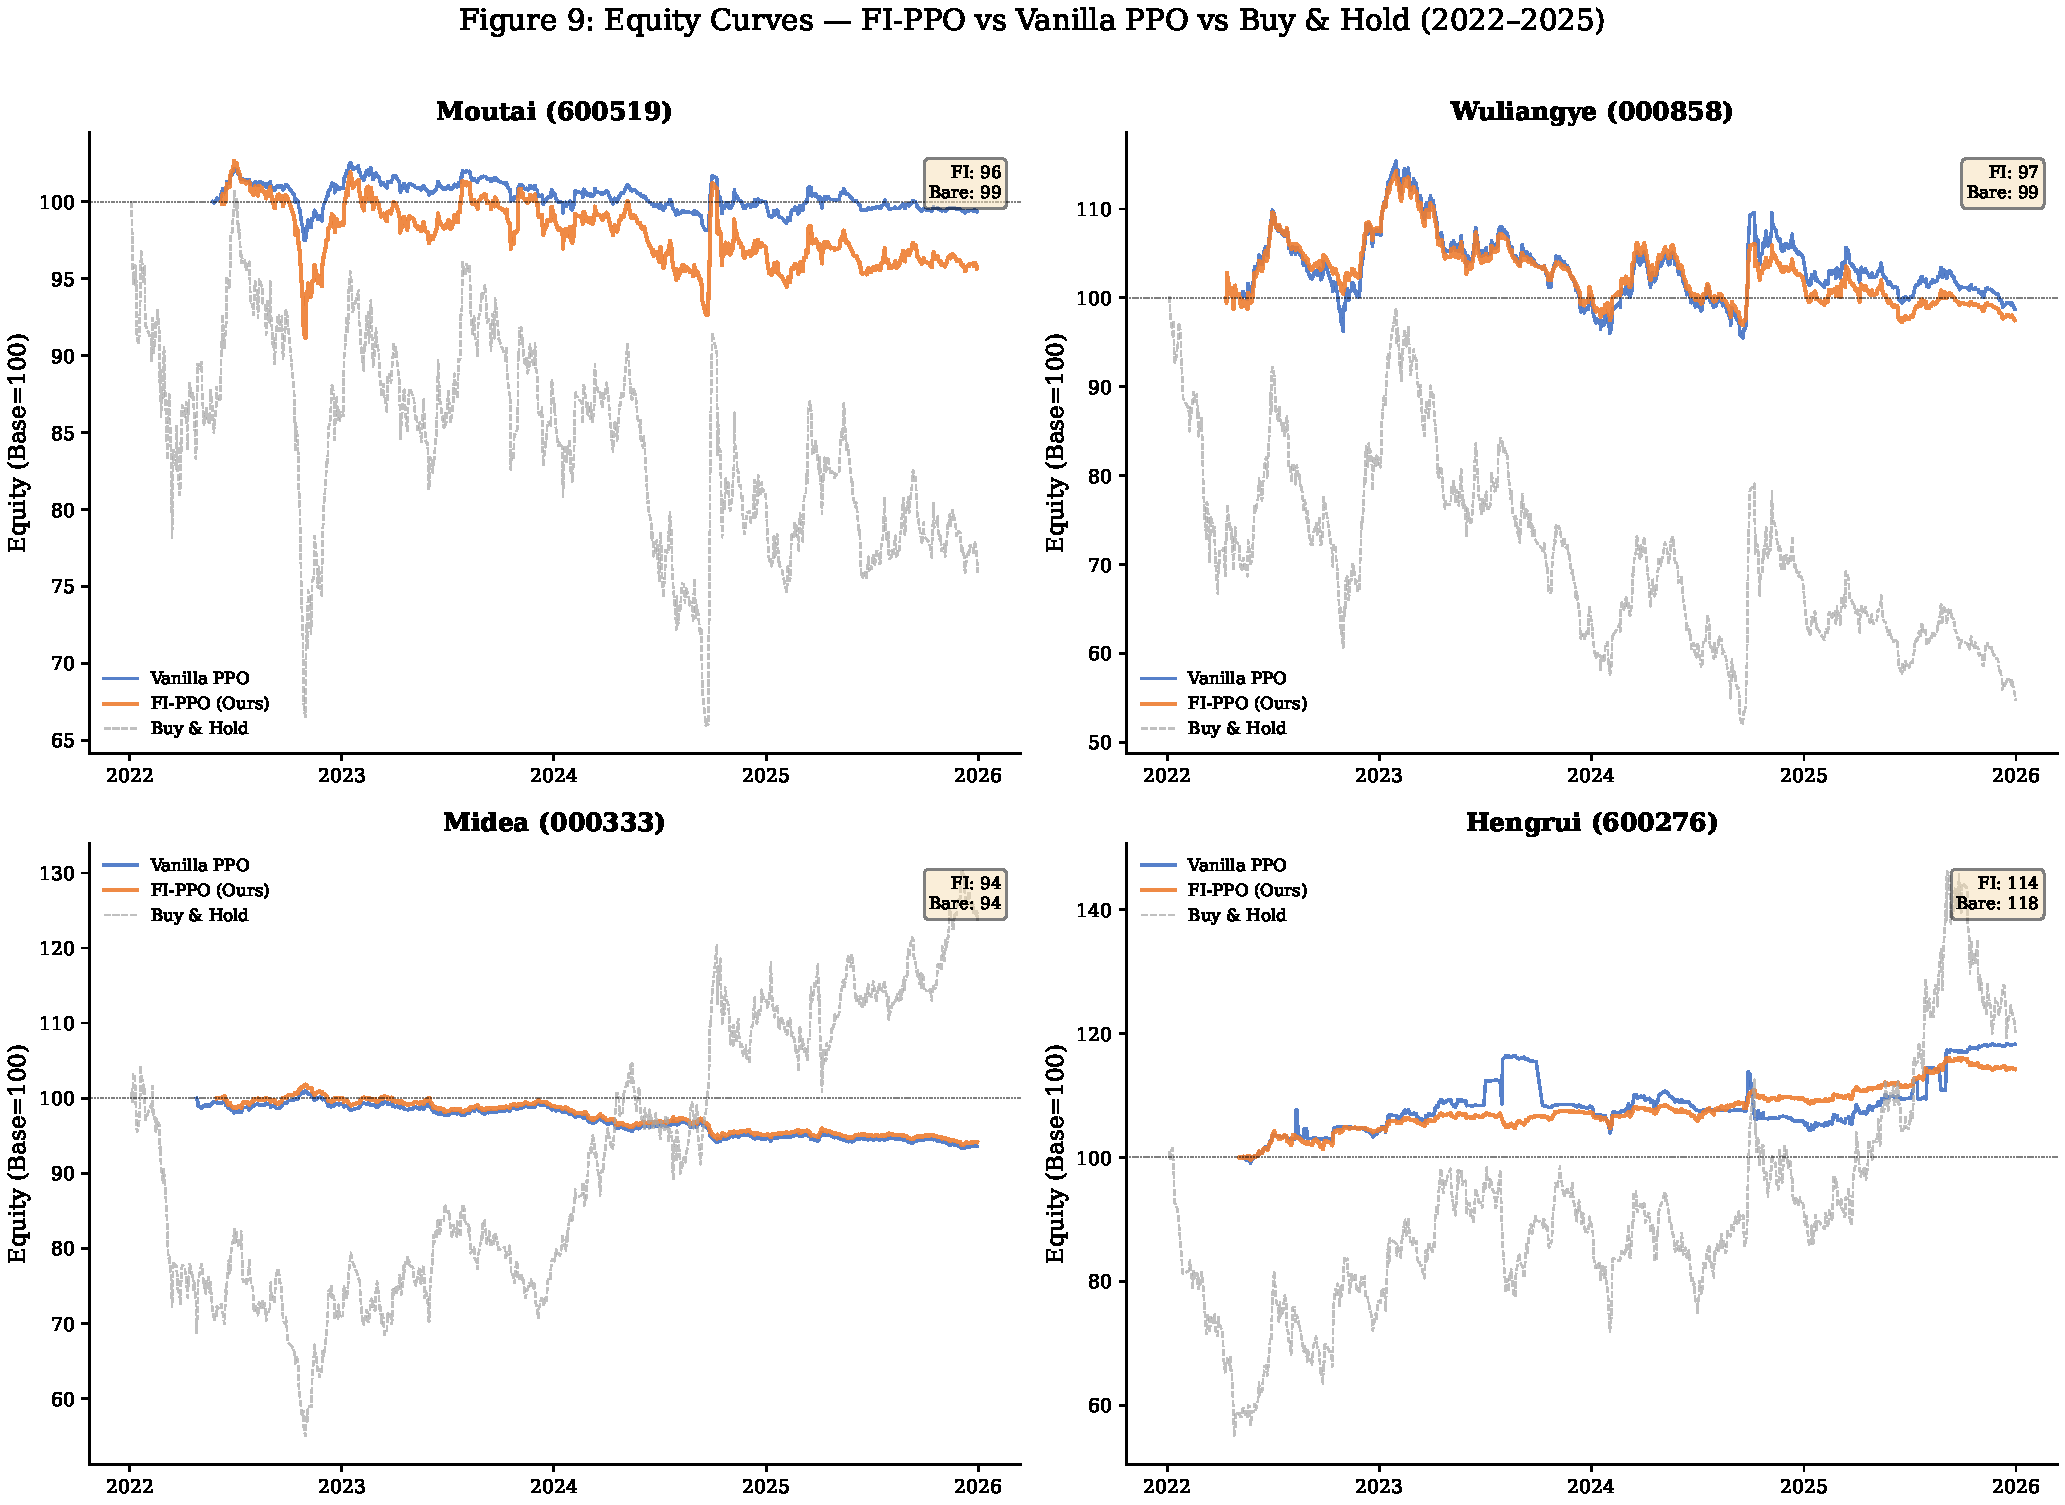
\includegraphics[width=\textwidth]{figures/fig9_equity_curves.pdf}
    \caption{Equity curves for four core stocks (2022--2025 test period). Each panel compares FI-PPO (orange), vanilla PPO (blue), and Buy\&Hold (gray dashed). Portfolio value is normalized to 100 at the start of the test period.}
    \label{fig:equity}
\end{figure}

\begin{figure}[H]
    \centering
    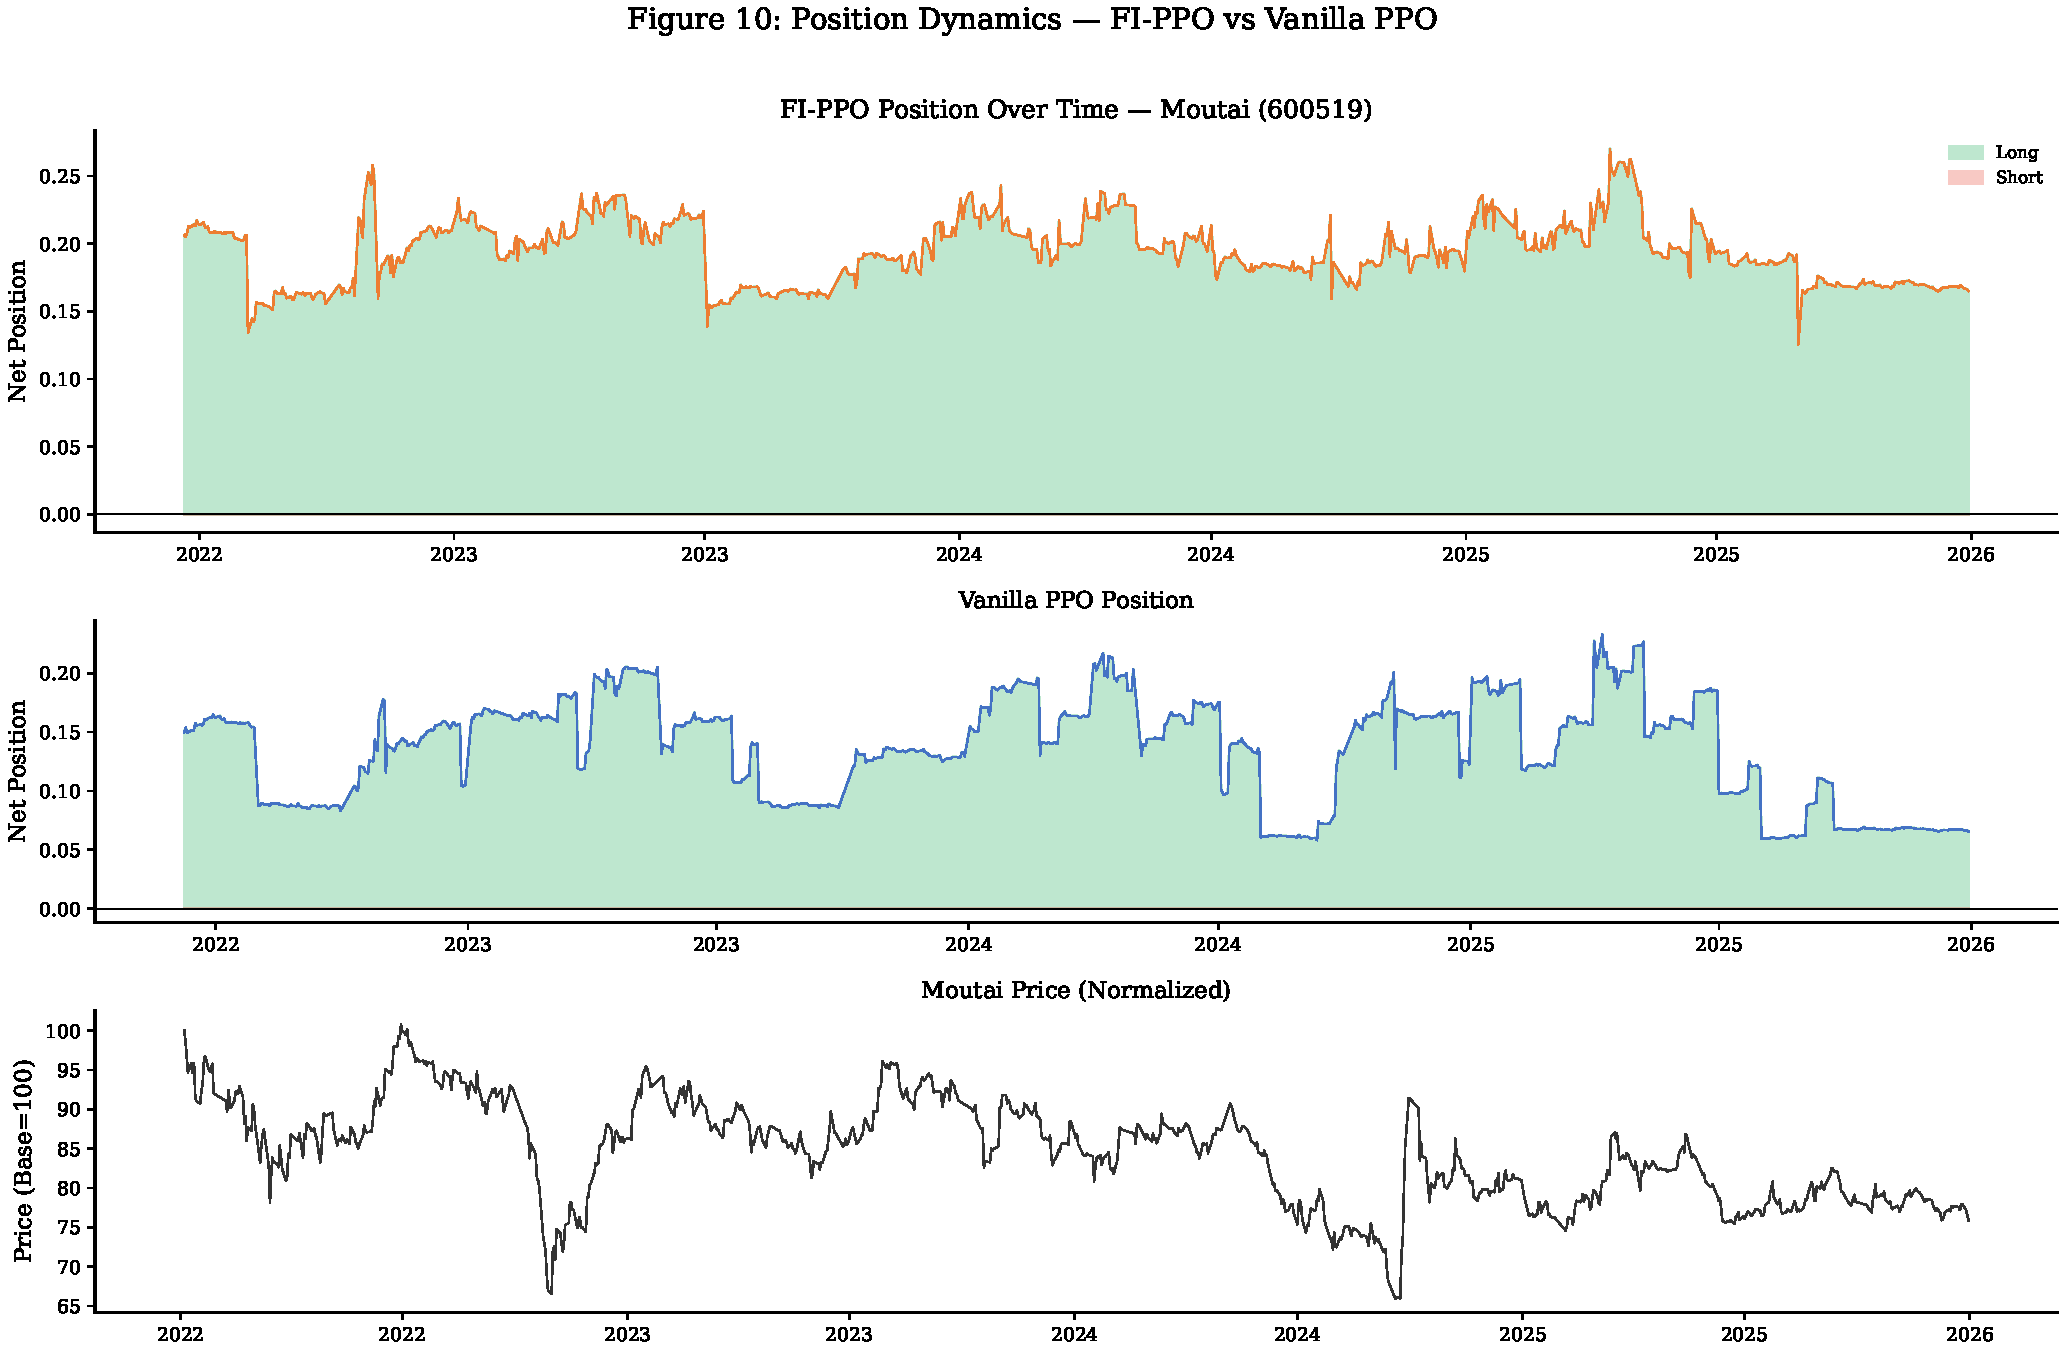
\includegraphics[width=\textwidth]{figures/fig10_positions.pdf}
    \caption{Position dynamics for Kweichow Moutai (600519). Top: FI-PPO net position showing active long/short management. Middle: Vanilla PPO net position. Bottom: Normalized stock price for context. Green shading indicates long exposure; red shading indicates short exposure.}
    \label{fig:positions}
\end{figure}

\end{document}
